\documentclass[aspectratio=169,t]{beamer}

% ---- Packages ----
\usepackage[T1]{fontenc}
\usepackage{graphicx}
\usepackage{amsmath,amssymb,amsthm}
\usepackage{booktabs}
\usepackage{array}
\usepackage{xcolor}
\usepackage{hyperref}
\usepackage{tikz}
\usepackage{lmodern}

% ---- Beamer setup ----
\usetheme{default}
\setbeamertemplate{navigation symbols}{}
\setbeamertemplate{footline}{%
  \hfill{\footnotesize\color{gray}\insertframenumber\,/\,\inserttotalframenumber\hspace{0.4cm}}\vspace{0.25cm}%
}
\setbeamersize{text margin left=0.7cm, text margin right=0.7cm}

% ---- Colors ----
\definecolor{accentred}{RGB}{204,51,51}
\definecolor{darkgray}{RGB}{80,80,80}

% ---- Beamer colors ----
\setbeamercolor{background canvas}{bg=white}
\setbeamercolor{normal text}{fg=black}
\setbeamercolor{frametitle}{fg=black}
\setbeamerfont{frametitle}{size=\large, series=\bfseries}
\setbeamercolor{itemize item}{fg=accentred}
\setbeamercolor{itemize subitem}{fg=accentred}
\setbeamercolor{enumerate item}{fg=accentred}
\setbeamercolor{block title}{fg=white, bg=accentred}
\setbeamercolor{block body}{fg=black, bg=red!8}

% ---- Frametitle with red underline ----
\setbeamertemplate{frametitle}{%
  \vspace{0.3cm}%
  \insertframetitle\par%
  \textcolor{accentred}{\rule{\textwidth}{1pt}}%
  \vspace{-0.1cm}%
}

% ---- Convenience macros ----
\newcommand{\includegraphicscenter}[2]{%
  \begin{center}
    \includegraphics[#1]{#2}
  \end{center}%
}

\newcommand {\framedgraphic}[2] {
    \begin{frame}{#1}
        \begin{center}
            \includegraphics[width=\textwidth,height=0.8\textheight,keepaspectratio]{#2}
        \end{center}
    \end{frame}
}

% ---- Section interlude macro ----
\newcommand{\sectionframe}[2][]{%
  \begingroup
  \setbeamercolor{background canvas}{bg=accentred}
  \setbeamertemplate{footline}{}%
  \begin{frame}[plain]
    \color{white}
    \vspace{2.0cm}
    {\LARGE\bfseries\raggedright #2}
    \ifx\relax#1\relax\else
      \vspace{0.5cm}
      {\normalsize\raggedright #1}
    \fi
  \end{frame}
  \endgroup
}


\coursetitle{Course: Foundations of AI with Embeddings}
\title{Lecture 1: Basic dimensionality reduction algorithms}
\subtitle{PCA \enspace$\cdot$\enspace MDS \enspace$\cdot$\enspace Local~MDS \enspace$\cdot$\enspace Isomap \enspace$\cdot$\enspace DBSCAN}
\author{Liubov Tupikina, Vladimir Kukushkin}
\institute{Constructor University}
\date{2026}

\begin{document}

\maketitle

% ============================================================
% OUTLINE
% ============================================================
\begin{frame}{Outline}
  \vspace{0.4cm}
  \begin{enumerate}
    \setlength{\itemsep}{0.4cm}
    \item Problem Statement
    \item Principal Component Analysis (PCA)
    \item Multidimensional Scaling (MDS)
    \item Local MDS and Isomap
    % \item DBSCAN Clustering
  \end{enumerate}
\end{frame}


% ============================================================
\sectionframe{1. Problem Statement}
% ============================================================

\begin{frame}{Problem Statement}
  \begin{itemize}
    \setlength{\itemsep}{0.4cm}
    \item We have data in a $p$-dimensional space --- too complex to visualise or analyse directly.
    \item We want to transform points from this high-dimensional space into a lower-dimensional subspace (e.g. 2D).
    \item Why?
    \begin{itemize}
      \item After reduction we can find and visualise clusters, detect outliers.
      \item Reducing noise in the data.
      \item Data compression.
    \end{itemize}
  \end{itemize}

  \vspace{0.5cm}
  \textbf{Key question:} How to choose the optimal projection?
\end{frame}


\begin{frame}{From $N \times p$ to $N \times q$}
  \vspace{0.15cm}
  \begin{center}
  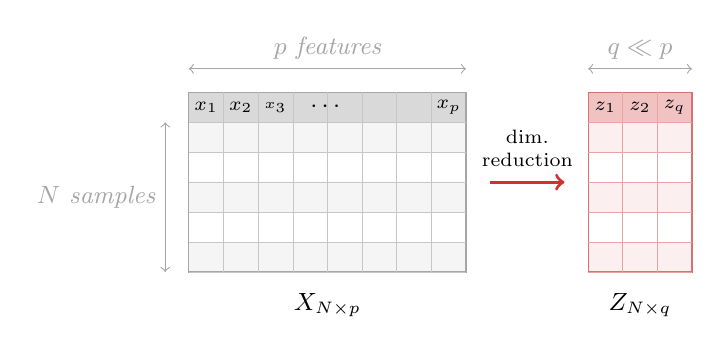
\begin{tikzpicture}[x=1cm, y=1cm]
    %% cell: cw=0.44, ch=0.38; p=8 cols, q=3 cols, N=5 data rows
    %% Left matrix : x in [0, 3.52],  header y in [0, 0.38], data y in [0, -1.90]
    %% Right matrix: x in [5.07, 6.39], same y range

    % ---- LEFT MATRIX (N x p) ----
    \fill[gray!30]  (0, 0)     rectangle (3.52,  0.38);
    \fill[gray!8]   (0, 0)     rectangle (3.52, -0.38);
    \fill[white]    (0,-0.38)  rectangle (3.52, -0.76);
    \fill[gray!8]   (0,-0.76)  rectangle (3.52, -1.14);
    \fill[white]    (0,-1.14)  rectangle (3.52, -1.52);
    \fill[gray!8]   (0,-1.52)  rectangle (3.52, -1.90);
    \draw[gray!70, thin] (0, 0.38) rectangle (3.52, -1.90);
    \foreach \j in {1,...,7} {
      \draw[gray!45, very thin] ({0.44*\j},  0.38) -- ({0.44*\j}, -1.90);
    }
    \foreach \i in {0,...,5} {
      \draw[gray!45, very thin] (0, {-0.38*\i}) -- (3.52, {-0.38*\i});
    }
    % column headers
    \node[font=\scriptsize] at (0.22, 0.19) {$x_1$};
    \node[font=\scriptsize] at (0.66, 0.19) {$x_2$};
    \node[font=\tiny]       at (1.10, 0.19) {$x_3$};
    \node[font=\small]      at (1.76, 0.19) {$\cdots$};
    \node[font=\scriptsize] at (3.30, 0.19) {$x_p$};
    % dimension arrows
    \draw[<->, gray!70, thin] (0, 0.68) -- (3.52, 0.68)
      node[midway, above, font=\small\itshape] {$p$ features};
    \draw[<->, gray!70, thin] (-0.30, 0) -- (-0.30, -1.90)
      node[midway, left, font=\small\itshape] {$N$ samples};
    \node[below, font=\small\bfseries] at (1.76, -2.05) {$X_{N \times p}$};

    % ---- ARROW ----
    \draw[->, very thick, accentred] (3.82, -0.76) -- (4.77, -0.76);
    \node[above, font=\scriptsize, align=center] at (4.30, -0.68)
      {dim.\\reduction};

    % ---- RIGHT MATRIX (N x q) ----
    \fill[accentred!30] (5.07, 0)     rectangle (6.39,  0.38);
    \fill[accentred!8]  (5.07, 0)     rectangle (6.39, -0.38);
    \fill[white]        (5.07,-0.38)  rectangle (6.39, -0.76);
    \fill[accentred!8]  (5.07,-0.76)  rectangle (6.39, -1.14);
    \fill[white]        (5.07,-1.14)  rectangle (6.39, -1.52);
    \fill[accentred!8]  (5.07,-1.52)  rectangle (6.39, -1.90);
    \draw[accentred!70, thin] (5.07, 0.38) rectangle (6.39, -1.90);
    \foreach \j in {1,...,2} {
      \draw[accentred!45, very thin] ({5.07+0.44*\j},  0.38) -- ({5.07+0.44*\j}, -1.90);
    }
    \foreach \i in {0,...,5} {
      \draw[accentred!45, very thin] (5.07, {-0.38*\i}) -- (6.39, {-0.38*\i});
    }
    % column headers
    \node[font=\scriptsize] at (5.29, 0.19) {$z_1$};
    \node[font=\scriptsize] at (5.73, 0.19) {$z_2$};
    \node[font=\scriptsize] at (6.17, 0.19) {$z_q$};
    % dimension arrows
    \draw[<->, gray!70, thin] (5.07, 0.68) -- (6.39, 0.68)
      node[midway, above, font=\small\itshape] {$q \ll p$};
    \node[below, font=\small\bfseries] at (5.73, -2.05) {$Z_{N \times q}$};

  \end{tikzpicture}
  \end{center}
  \vspace{0.15cm}
  \begin{center}
    {\small\itshape
      $X$ --- original data matrix;\quad
      $Z$ --- low-dimensional representation;\quad
      each \textbf{row} is one sample}
  \end{center}
\end{frame}


% ============================================================
\sectionframe{2. Principal Component Analysis (PCA)}
% ============================================================

\begin{frame}{PCA --- Idea}
  \begin{itemize}
    \setlength{\itemsep}{0.4cm}
    \item \textbf{Informativeness $\approx$ variance.}
          A feature with constant values carries no information and can be discarded.
    \item We want to project data onto a subspace where the variance along
          each basis direction is \textbf{maximised}.
    \item The dimensionality $q$ of the target subspace is a hyperparameter
          chosen by the user.
  \end{itemize}
\end{frame}

\begin{frame}[shrink=5]{Variance along an axis}
  \begin{columns}[T]
    \column{0.57\textwidth}
    \vspace{0.1cm}
    Let $v\in \mathbb{R}^p$ be a unit vector we project onto. Then
    \begin{itemize}
      \setlength{\itemsep}{0.2cm}
      \item $\theta_i := \|z_i\| = \frac{v^T\cdot x_i}{\|v\|} = v^T\cdot x_i$
      \item $Var(\theta) := \frac{1}{N} \sum_{i=1}^N (\theta_i - \bar{\theta})^2 = \frac{1}{N} \sum_{i=1}^N (v^T\cdot x_i - \bar{\theta})^2$
      \item Assume that $\bar \theta = 0$ (we can always subtract the mean from the data).
      \item $Var(\theta) = \frac{1}{N} \sum_{i=1}^N (v\cdot x_i)^2 = \frac{1}{N} (Xv)^T (Xv) = v^T \Sigma v$,\\
            where $\Sigma = \frac{1}{N} X^T X$ is the covariance matrix.
    \end{itemize}

    \vspace{0.2cm}
    Therefore:
    \[
      \hat v = \arg\max_{v} v^T \Sigma v
    \]

    \column{0.43\textwidth}
    \vspace{0.4cm}
    \begin{center}
    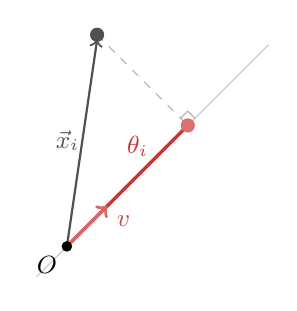
\begin{tikzpicture}[scale=1.28]
      % Projection axis in w direction (45°)
      \draw[gray!40, thin] (-0.3,-0.3) -- (2.0,2.0);
      % x_i vector from origin
      \draw[->, thick, darkgray] (0,0) -- (0.3,2.05);
      \node[darkgray, left, font=\small] at (0.22,1.05) {$\vec{x}_i$};
      % Dashed perpendicular from x_i to foot
      \draw[dashed, gray!60, thin] (0.3,2.1) -- (1.2,1.2);
      % Right-angle mark at foot (1.2,1.2):
      %   step along w   = 0.10*(0.707, 0.707) = (0.071, 0.071)
      %   step along perp= 0.10*(-0.707, 0.707) = (-0.071, 0.071)
      \draw[gray!65, thin]
        (1.271,1.271) -- (1.200,1.342) -- (1.129,1.271);
      % θ_i: projection segment from O to foot
      \draw[accentred, very thick] (0,0) -- (1.2,1.2);
      \node[accentred, font=\small\bfseries, above left] at (0.9,0.8) {$\theta_i$};
      % w unit vector arrow
      \draw[->, very thick, accentred!75] (0,0) -- (0.4,0.4);
      \node[accentred!90, font=\small\bfseries, below right] at (0.4,0.4) {$v$};
      % Points
      \fill[accentred!70] (1.2,1.2) circle (2.0pt);
      \fill[darkgray]     (0.3,2.1) circle (2.0pt);
      \fill[black]        (0,0)     circle (1.5pt);
      \node[below left, font=\small] at (0,0) {$O$};
    \end{tikzpicture}
    \end{center}
  \end{columns}
\end{frame}

\begin{frame}{PCA: Solution}
  \begin{columns}[c]
    \column{0.52\textwidth}
    \vspace{0.1cm}
    \begin{center}
    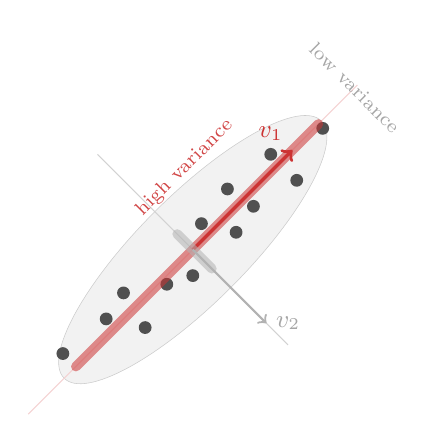
\begin{tikzpicture}[scale=1.1]
      % Cloud envelope
      \fill[gray!10, rotate=45] (0,0) ellipse (2.1cm and 0.62cm);
      \draw[gray!40, very thin, rotate=45] (0,0) ellipse (2.1cm and 0.62cm);
      % Extended direction lines (faint background)
      \draw[accentred!22, thin] (-1.9,-1.9) -- (1.9,1.9);
      \draw[gray!35, thin]      (-1.1, 1.1) -- (1.1,-1.1);
      % Data points
      \foreach \px/\py in {
          -1.5/-1.2, -1.0/-0.8, -0.55/-0.9, -0.3/-0.4,
           0.1/0.3,   0.5/0.2,   0.4/0.7,   0.9/1.1,
           1.2/0.8,   1.5/1.4,  -0.8/-0.5,  0.0/-0.3, 0.7/0.5}
      { \fill[darkgray] ({\px},{\py}) circle (2.1pt); }
      % Spread bar on v1 (long red segment = large variance)
      \draw[accentred, line width=3.5pt, opacity=0.55, line cap=round]
        (-1.35,-1.35) -- (1.45,1.45);
      \node[accentred!90, font=\scriptsize, rotate=45, above=2pt]
        at (0.1, 0.75) {high variance};
      % v1 arrow + label
      \draw[->, very thick, accentred] (0,0) -- (1.15,1.15);
      \node[accentred, font=\small\bfseries, above left] at (1.15,1.15) {$v_1$};
      % Spread bar on v2 (short gray segment = small variance)
      \draw[gray!60, line width=3.5pt, opacity=0.55, line cap=round]
        (-0.18, 0.18) -- (0.22,-0.22);
      \node[gray!70, font=\scriptsize, rotate=-45, below=2pt]
        at (2.05, 2.05) {low variance};
        % at (0.52, 0.05) {low variance};
      % v2 arrow + label
      \draw[->, thick, gray!60] (0,0) -- (0.85,-0.85);
      \node[gray!70, font=\small\bfseries, right] at (0.85,-0.85) {$v_2$};
    \end{tikzpicture}
    \end{center}

    \column{0.48\textwidth}
    \vspace{0.1cm}

    \textbf{Solution:} leading $q$ eigenvectors of $\Sigma$:
    $$\Sigma\, \hat v_1 = \lambda_1\, \hat v_1,$$
    $$\cdots$$
    $$\Sigma\, \hat v_q = \lambda_q\, \hat v_q,$$
    where $\lambda_1 \geq \lambda_2 \geq \cdots \geq \lambda_q$.

    \vspace{0.3cm}
    \textbf{For $q$ axes:}
    top-$q$ eigenvectors (mutually orthogonal).
  \end{columns}
\end{frame}

\begin{frame}{A case study: handwritten digits}
  \begin{itemize}
      \item 130 hadwritten threes.
      \item Each image is of $16\times 16 = 256$ pixels. Feature is a pixel's grayscale value (0..255). 
  \end{itemize}
  \includegraphicscenter{height=0.65\textheight}{img/pca_threes_1.png}
\end{frame}

\framedgraphic{Shortcomings of global approaches}{img/pca_threes_2.png}

% ============================================================
\sectionframe{3. Multidimensional Scaling (MDS)}
% ============================================================

\begin{frame}{MDS --- Idea}
  \begin{itemize}
    \setlength{\itemsep}{0.35cm}
    \item Often we only care about preserving \textbf{pairwise distances}, not the absolute coordinates.
    \item MDS finds $N$ points $z_1, \ldots, z_N \in \mathbb{R}^q$ minimising the \textbf{stress function}:
    \[
      S_M(z_1,\ldots,z_N)
      = \sum_{i < i'} \bigl(d_{ii'} - \|z_i - z_{i'}\|\bigr)^2
      \tag{3}
    \]
    where $d_{ii'}$ are the original pairwise distances.
    \item MDS is a \textbf{non-linear} method (despite a linear-algebra solution for classical MDS).
  \end{itemize}
\end{frame}

\begin{frame}{MDS --- Similarity-Based Variant}
  In practice, distances can be replaced by \textbf{similarities}:
  \[
    s_{ii'} = \langle x_i - \bar{x},\; x_{i'} - \bar{x} \rangle,
  \]
  and the stress becomes:
  \[
    S_C(z_1,\ldots,z_N)
    = \sum_{i < i'} \bigl(s_{ii'} - \langle z_i - \bar{z},\; z_{i'} - \bar{z}\rangle\bigr)^2.
  \]

  \vspace{0.3cm}
  \begin{columns}[T]
    \column{0.5\textwidth}
    \textcolor{accentred}{\bfseries Strengths}
    \begin{itemize}
      \item Non-linear method
      \item Preserves \textbf{global} pairwise (Euclidean) distances
    \end{itemize}

    \column{0.5\textwidth}
    \textcolor{accentred}{\bfseries Limitations}
    \begin{itemize}
      \item Still uses global Euclidean distances
      \item Does not capture \textbf{local} structure of the manifold
      \item Sensitive to outliers in the distance matrix
    \end{itemize}
  \end{columns}
\end{frame}


% ============================================================
\sectionframe{4. Local MDS and ISOMAP}
% ============================================================

\begin{frame}{Motivation: Global vs.\ Local Structure}
  \begin{itemize}
    \setlength{\itemsep}{0.4cm}
    \item PCA and MDS preserve \textbf{global} Euclidean distances.
    \item For data lying on a \textbf{curved manifold}, Euclidean distances are misleading: two points on opposite sides of a roll are \emph{far} along the surface but \emph{close} in Euclidean space.
    \item We want methods that respect the \textbf{intrinsic geometry} of the data.
  \end{itemize}

  \vspace{0.5cm}
  \begin{block}{Idea}
    Replace Euclidean distances with distances that follow the shape of the manifold.
  \end{block}
\end{frame}

\framedgraphic{Shortcomings of global approaches}{img/mds.png}

\begin{frame}{Local MDS}
  Let $\mathcal{N}$ be the set of \emph{neighbour pairs}:
  $(i,i') \in \mathcal{N}$ iff $i'$ is among the $K$ nearest neighbours of $i$.

  \vspace{0.25cm}
  Modified stress function:
  \[
    S_L = \underbrace{\sum_{(i,i')\in\mathcal{N}} \!\!(d_{ii'} - \|z_i - z_{i'}\|)^2}_{\text{local: preserve neighbour distances}}
        + w \underbrace{\sum_{(i,i')\notin\mathcal{N}} \!\!(D - \|z_i - z_{i'}\|)^2}_{\text{repulsion: push non-neighbours apart}}
  \]
  where $D$ is a large constant and $w$ is a weight.

  \vspace{0.25cm}
  \textbf{Practical relaxation} (replacing the repulsion term):
  \[
    S_L \approx \sum_{(i,i')\in\mathcal{N}} (d_{ii'} - \|z_i - z_{i'}\|)^2
              + \tau \!\!\sum_{(i,i')\notin\mathcal{N}} \|z_i - z_{i'}\|,
  \]
  where $\tau = 2wD$ is a tunable regularisation parameter.
\end{frame}

\begin{frame}{ISOMAP}
  \begin{enumerate}
    \setlength{\itemsep}{0.4cm}
    \item \textbf{Build a neighbourhood graph.}
          Connect each point to its $K$ nearest neighbours (or all points within radius $\varepsilon$).
          Edge weights = Euclidean distances.

    \item \textbf{Compute geodesic distances.}
          Shortest-path distances on the graph (e.g.\ via Dijkstra's algorithm)
          approximate \emph{manifold} distances $d_{ii'}$.

    \item \textbf{Apply MDS.}
          Use the geodesic distance matrix as input to standard MDS.
  \end{enumerate}

\end{frame}

\framedgraphic{ISOMAP}{img/isomap.png}

\begin{frame}{Beyond Isomap: Modern Manifold Methods}
  \begin{columns}[T]
    \column{0.5\textwidth}
    \textcolor{accentred}{\bfseries t-SNE}
    \hfill{\small van der Maaten \& Hinton, 2008}
    \begin{itemize}
      \setlength{\itemsep}{0.25cm}
      \item Accounts for \textbf{local density}, not just distances
      \item Very effective for 2D/3D visualisation
      \item \textbf{Slow:} $\mathcal{O}(N^2)$ --- scales poorly
    \end{itemize}

    \column{0.5\textwidth}
    \textcolor{accentred}{\bfseries UMAP}
    \hfill{\small McInnes et al., 2018}
    \begin{itemize}
      \setlength{\itemsep}{0.25cm}
      \item Preserves both \textbf{local and global} structure
      \item Stronger theoretical foundations (topology)
      \item \textbf{Faster} and more scalable than t-SNE
    \end{itemize}
  \end{columns}

  \vspace{0.7cm}
  \begin{center}
    {\small These methods will be covered in detail in the next lectures.}
  \end{center}
\end{frame}


% % ============================================================
% \sectionframe{5. DBSCAN}
% % ============================================================

% \begin{frame}{DBSCAN --- Motivation}
%   \begin{itemize}
%     \setlength{\itemsep}{0.4cm}
%     \item Isomap and Local MDS capture local structure --- but they are
%           \textbf{dimensionality reduction} methods, not clustering methods.
%     \item We want a \textbf{clustering} algorithm with similar local awareness.
%     \item Classical methods (e.g.\ $k$-means) assume \textbf{convex, ball-shaped} clusters ---
%           inadequate for complex geometries.
%     \item Goal: distinguish \textbf{core points} (in dense regions) from
%           \textbf{border points} and \textbf{noise}.
%   \end{itemize}
% \end{frame}

% \begin{frame}{DBSCAN --- Definitions}
%   \textbf{Parameters:}
%   $\varepsilon$ (neighbourhood radius), $\mathrm{minPts}$ (minimum neighbourhood size).

%   \vspace{0.3cm}
%   \begin{itemize}
%     \setlength{\itemsep}{0.3cm}
%     \item $N_\varepsilon(p)$ --- all points within distance $\varepsilon$ of $p$ (including $p$).
%     \item Point $p$ is a \textbf{core point} if $|N_\varepsilon(p)| \geq \mathrm{minPts}$.
%     \item Point $q$ is \textbf{directly reachable} from $p$
%           if $q \in N_\varepsilon(p)$ and $p$ is a core point.
%     \item Point $q$ is \textbf{reachable} from $p$ if there exists a chain
%           $p_1 = p,\, p_2,\, \ldots,\, p_n = q$ where each $p_{k+1}$
%           is directly reachable from $p_k$.
%     \item Points not reachable from any core point are \textbf{outliers (noise)}.
%   \end{itemize}
% \end{frame}

% \begin{frame}{DBSCAN --- Algorithm}
%   \begin{columns}[T]
%     \column{0.55\textwidth}
%     \vspace{0.2cm}
%     \begin{enumerate}
%       \setlength{\itemsep}{0.3cm}
%       \item Mark all points as \emph{unvisited}.
%       \item Pick an unvisited point $p$; mark it visited.
%       \item If $|N_\varepsilon(p)| < \mathrm{minPts}$,
%             tentatively label $p$ as \textbf{noise}.
%       \item Otherwise, start a new cluster; add all points in
%             $N_\varepsilon(p)$ to it and expand recursively.
%       \item Repeat until all points are visited.
%     \end{enumerate}

%     \column{0.45\textwidth}
%     \vspace{0.2cm}
%     \begin{block}{Example ($\mathrm{minPts} = 4$)}
%       \begin{itemize}
%         \item \textcolor{red}{\bfseries Red}: core points
%         \item \textcolor{orange}{\bfseries Yellow}: border points
%               (reachable from cores)
%         \item \textcolor{blue}{\bfseries Blue}: outliers / noise
%       \end{itemize}
%     \end{block}
%   \end{columns}
% \end{frame}

% \begin{frame}{DBSCAN --- Pros and Cons}
%   \begin{columns}[T]
%     \column{0.5\textwidth}
%     \textcolor{accentred}{\bfseries Advantages}
%     \begin{itemize}
%       \setlength{\itemsep}{0.3cm}
%       \item Finds clusters of \textbf{arbitrary shape}
%       \item \textbf{No need} to specify the number of clusters
%       \item \textbf{Robust} to outliers --- identifies them explicitly
%     \end{itemize}

%     \column{0.5\textwidth}
%     \textcolor{accentred}{\bfseries Limitations}
%     \begin{itemize}
%       \setlength{\itemsep}{0.3cm}
%       \item Must choose $\varepsilon$ and $\mathrm{minPts}$
%       \item Requires a \textbf{distance metric} for $\varepsilon$-neighbourhoods
%       \item \textbf{Ambiguity} at cluster boundaries
%       \item Struggles with \textbf{varying density} clusters
%       \item Complexity: $\mathcal{O}(N \log N)$ with spatial indexing
%     \end{itemize}
%   \end{columns}
% \end{frame}


% ============================================================
% REFERENCES
% ============================================================
\begin{frame}{References}
  \small
  \begin{thebibliography}{9}
    \bibitem{golub}
      Golub, G.H., Van Loan, C.F.
      \textit{Matrix Computations}.
      Johns Hopkins University Press, 4th ed., 2013.

    \bibitem{esl}
      Hastie, T., Tibshirani, R., Friedman, J.
      \textit{The Elements of Statistical Learning}.
      Springer, 2nd ed., 2009.

    \bibitem{isomap}
      Tenenbaum, J.B., de Silva, V., Langford, J.C.
      ``A global geometric framework for nonlinear dimensionality reduction.''
      \textit{Science}, 290(5500), 2000.

    \bibitem{dbscan}
      Ester, M., Kriegel, H.-P., Sander, J., Xu, X.
      ``A density-based algorithm for discovering clusters in large spatial databases.''
      \textit{KDD-96}, 1996.

    \bibitem{localmds}
      Chen, L., Buja, A.
      ``Local multidimensional scaling for nonlinear dimension reduction,
        graph drawing, and proximity analysis.''
      \textit{Journal of the American Statistical Association},
      104(485), 2009.
  \end{thebibliography}
\end{frame}


\end{document}
